\chapter{序論}


\section{Mg合金}
マグネシウム(Mg)は実用金属中において最も軽量かつ最大の振動吸収性をもつため, 航空機や自動車, 鉄道車両のフレーム, 工作機械で使用されるプーリーやロボットの骨格への応用が進められている. また,  Mg は海水中のにがりの主成分として含まれており日本国内においても十分に自給可能な金属である. このようなことから近年注目を集め, 様々な Mg 合金の研究開発が進められている. しかし,水やアルコールとよく反応してしまうため耐食性が悪く, Mg は 550〜600 $^\circ$C で発火するため大気中で火がつく可能性がある. それゆえ, 軽量金属であるアルミニウム(Al)合金に比べて実用が進んでいなかった.
しかし近年, Mg 合金において, LPSO 構造という新たな原子配列構造を持つ合金が開発された\cite{Th}. この Mg 合金は超々ジュラルミンの 1.2 倍の比降伏強度で, かつ難燃性であるという従来の常識を覆すような特性が得られている.


\section{LPSO 構造}
\subsection{積層欠陥}
積層欠陥とは積層順序の連続性が局所的に乱れた欠陥である. 図\ref{fig1}に hcp 構造の積層欠陥の様子を表した模式図を示した. hcp 構造ではこの図で示すように [0001] 方向に最密面が ABAB と積層しており, 赤枠で囲った原子を赤矢印の方向にずらすと, 積層順序が ABCA となる. その際に赤の破線で示した部分が積層欠陥面となる. そして hcp 構造上に発生した積層欠陥面の上下の黄丸で示した層を中心とした積層順序を考えると, それぞれ ABC,BCA となっている. このことから hcp 構造において積層欠陥が発生すると cubic 構造である fcc 構造が導入されることがわかる.

\begin{figure}[htbp]
	\begin{center}
		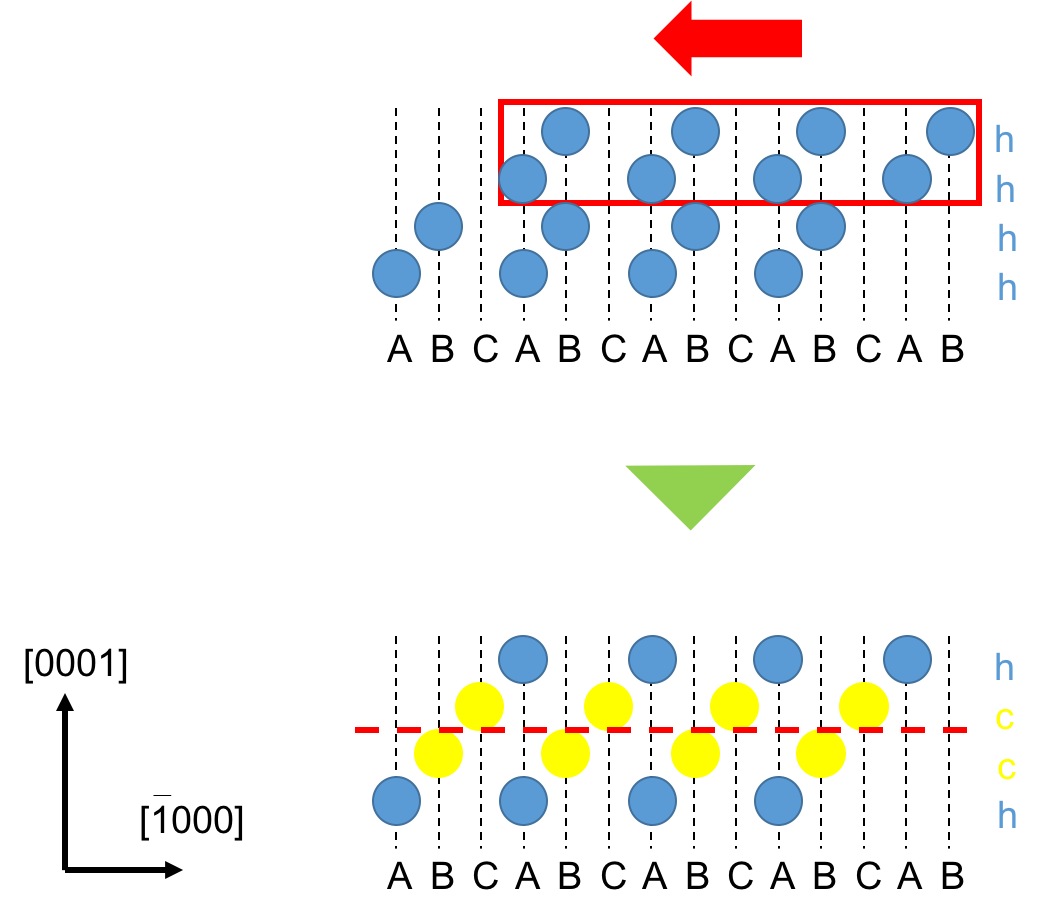
\includegraphics[width=100mm]{../intro/stuc.png}
		\caption{hcp 構造の積層欠陥の様子を表した模式図. 青丸は hexgonal 構造, 黄丸は cubic 構造を示している. また赤の破線部は積層欠陥部を示している.}
		\label{fig1}
	\end{center}
\end{figure}

\subsection{LPSO 構造}
LPSO ( Long Period Stacking Order ) 構造はその名称が示す通り,長周期の積層欠陥を含んだ構造であり,その積層欠陥部に溶質原子が濃化していることが研究の初期に判明していた. しかし, 液相から直接生成する合金系や, 固相から時効析出によって生成する系など多くの系で微妙に異なる構造を示すことが報告された. LPSO-Mg では下記の特徴がある.

\begin{itemize}
  \item $[0001]$ 方向において中周期的に積層欠陥が導入されている.
  \item 積層欠陥部には溶質原子であるZn,Yが集まっている.
  \item 集まった溶質原子が積層欠陥部において L1$_2$ クラスターを形成している.
\end{itemize}


\subsection{LPSO構造生成シナリオ}
西谷研究室では, 生成メカニズムに関するシナリオを立て, それらの実現可能性を第一原理計算によりエネルギー的に検証してきた. 当初は, 以下の 2 つのシナリオが立てられた.

\begin{itemize}
 \item 積層欠陥先行型
    \begin{itemize}
      \item hcp 構造の Mg において, 周期的に積層欠陥が導入される.
      \item 積層欠陥に溶質原子が捕まる.
     \end{itemize}
 \item 溶質原子先行型
 \begin{itemize}
      \item 積層欠陥が溶質原子を捕まえる.
      \item 積層欠陥から4層ほど離れた位置で溶質原子が濃化する.
	 \item 濃化した溶質原子が新たな積層欠陥を誘起する.
     \end{itemize}

\end{itemize}

\section{拡散}
\subsection{空孔拡散}
結晶中には原子の存在しない格子点があり, これを空孔(vacancy)という. 空孔と隣接する原子が位置を交換することにより拡散が起こる.
完全なカバレッジに近づく高いカバレッジレベルでの表面拡散の主な方法として起こり得る. このプロセスは、スライディングパズルで周りを滑るような方法に似ている. 高い拡散速度と低い空孔濃度のために、空孔拡散を直接観察することは非常に困難である. また, 単空孔と複空孔の拡散の模式図を図\ref{fig2}, 図\ref{fig3}に示した. 単空孔よりも複空孔の方が拡散の可能性が高くなる. それは図\ref{fig2}において赤線の山で表現している activation barrier 単空孔のほうが高いのが原因である.

\begin{figure}[htbp]
	\begin{center}
		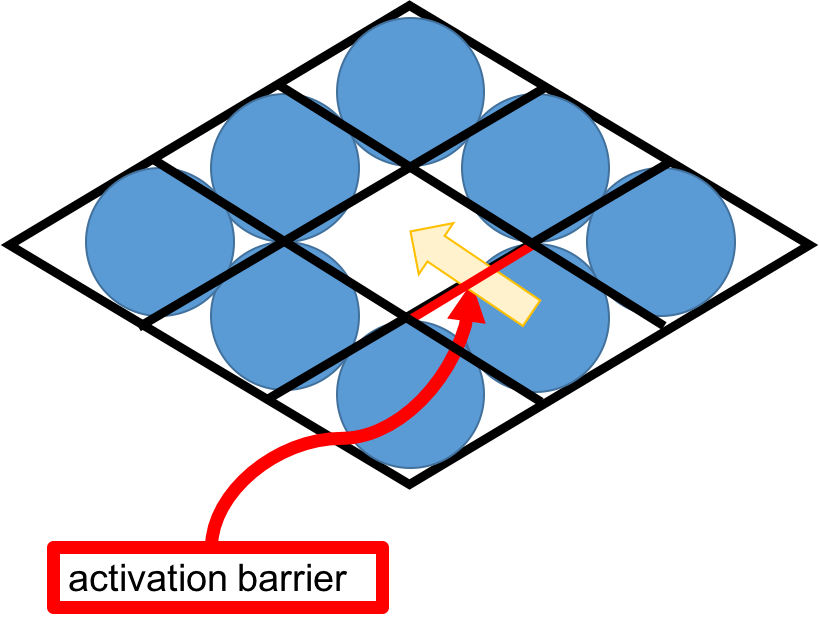
\includegraphics[width=80mm]{../intro/monovacancy.png}
        \caption{単空孔の拡散の模式図.}
		\label{fig2}
	\end{center}
\end{figure}

\begin{figure}[htbp]
	\begin{center}
		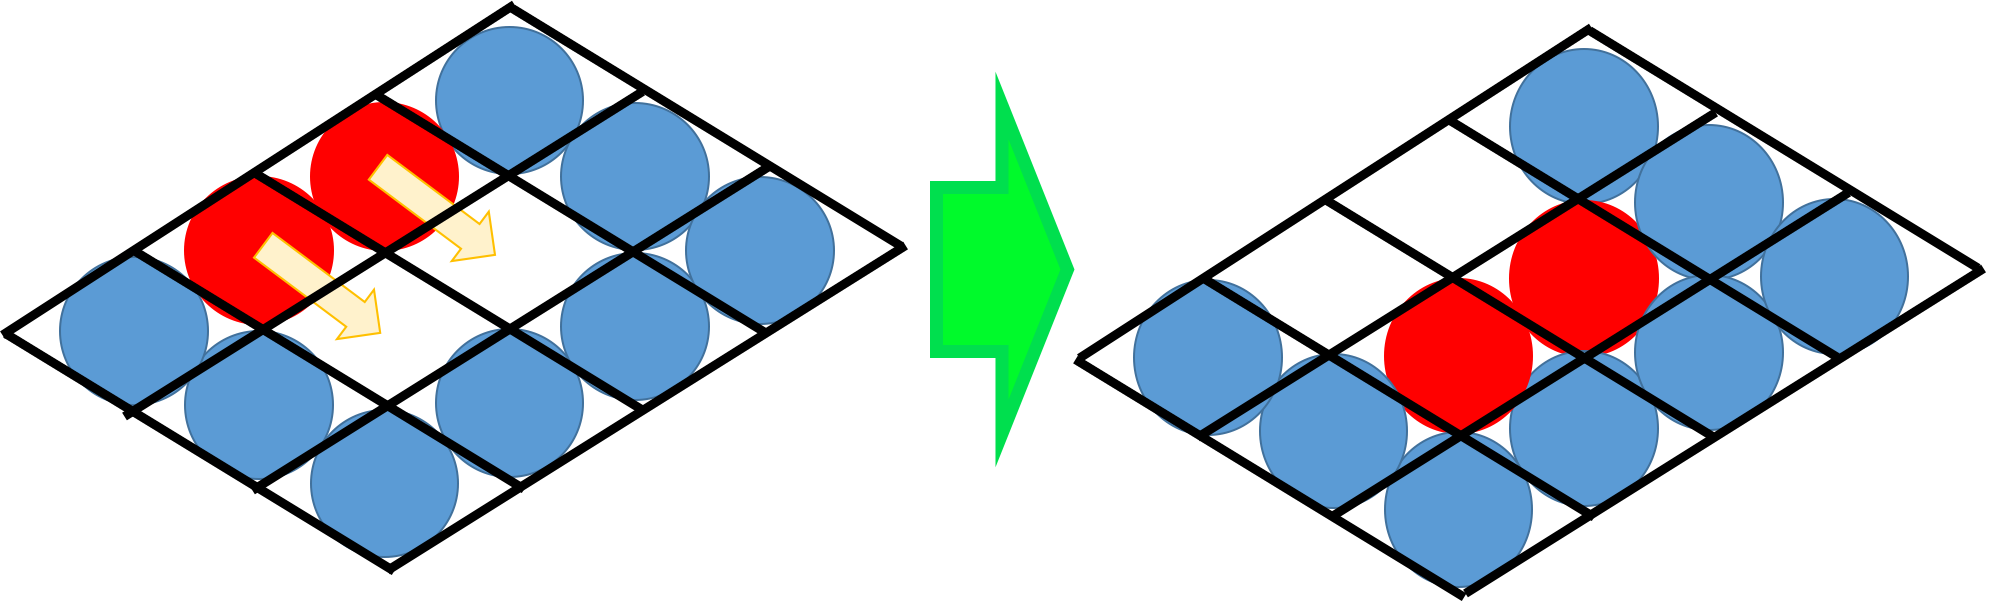
\includegraphics[width=130mm]{../intro/divacancy.png}
        \caption{複空孔の拡散の模式図.}
		\label{fig3}
	\end{center}
\end{figure}


\subsection{クラスター拡散}
クラスター拡散とは複数の原子の塊の移動のことを言う. クラスターの動きは、個々の原子, クラスターのセクション, またはクラスター全体が移動する場合がある.
クラスター拡散に関して, 結晶の表面では可能であるが, バルクでは不可能である.
理由は図\ref{fig4}で示すように表面では上層がないため動くことが可能だが, 図\ref{fig5}のようなバルクでは上層も原子が詰まっており動くことができないからである.

\begin{figure}[htbp]
	\begin{center}
		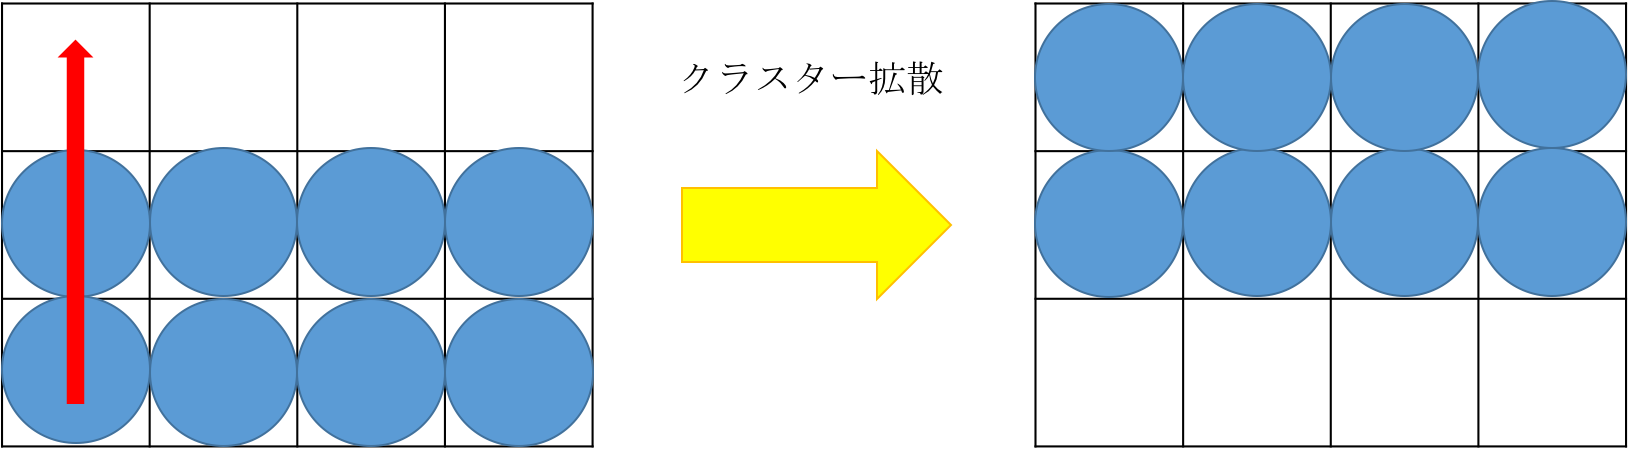
\includegraphics[width=100mm]{../intro/kakusan.png}
		\caption{クラスター拡散の模式図.}
		\label{fig4}
	\end{center}
\end{figure}

\begin{figure}[htbp]
	\begin{center}
		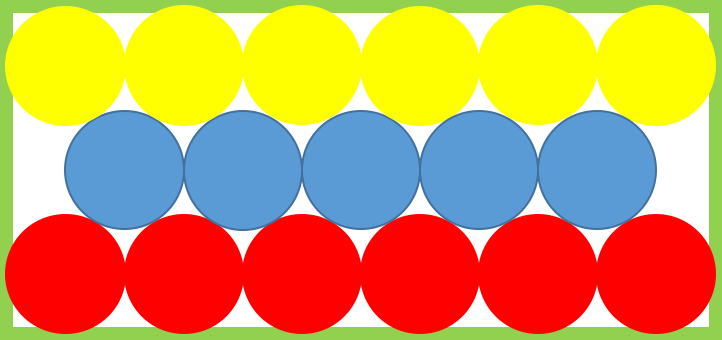
\includegraphics[width=70mm]{../intro/balc.png}
        \caption{バルク内の模式図.}
		\label{fig5}
	\end{center}
\end{figure}

\section{構造緩和}
構造緩和とは, 原子, または原子の集団を移動させて, 最安定構造を見つける事である. 本研究で行う構造緩和は, 結晶中の各原子を個々に移動させる内部緩和と, 格子定数を変化させて結晶格子の構造自体を緩和させる外部緩和を用いて最安定構造を求め, エネルギー値を算出する.

